\documentclass{article}
\usepackage{latexsym}
\usepackage{amssymb}
\usepackage{graphicx}
\usepackage{gensymb}
\usepackage[margin=1.2in]{geometry}
\usepackage{float}
\usepackage{wrapfig}
\usepackage{amsthm}
\usepackage{blkarray}
\usepackage{amsmath}
\usepackage{mathtools}
\usepackage{tikz}
\usepackage{framed}
\usepackage{fancyhdr}
\setcounter{page}{0}
\fancypagestyle{plain}{%
\pagestyle{fancy}
\fancyhf{}
\rhead{Tom Goodman}
\lhead{\leftmark}
\chead{}
\cfoot{\thepage} 
\renewcommand{\footrulewidth}{2pt}}
\pagestyle{plain}
\newcounter{thrmcount}[section]
\usepackage{listings}
    
\usepackage{graphicx}
    \graphicspath{ {/home/txg523/Desktop/Tex} }
    
    \newenvironment{thrm}
	{\begin{leftbar}\noindent\ignorespaces\textbf{Theorem \arabic{section}.\arabic{thrmcount}.}\par\noindent\ignorespaces}		
	{\end{leftbar}\stepcounter{thrmcount}\noindent\ignorespaces}
\newenvironment{lem}
	{\begin{leftbar}\noindent\ignorespaces\textbf{Lemma \arabic{section}.\arabic{thrmcount}.}\par\noindent\ignorespaces}		
	{\end{leftbar}\stepcounter{thrmcount}\noindent\ignorespaces}
\newenvironment{nthrm}[1]	
	{\begin{leftbar}\noindent\ignorespaces\textbf{Theorem \arabic{section}.\arabic{thrmcount}.} \textit{(#1)}\par\noindent\ignorespaces}
	{\end{leftbar}\stepcounter{thrmcount}\noindent\ignorespaces}
\newenvironment{nlem}[1]
	{\begin{leftbar}\noindent\ignorespaces\textbf{Lemma \arabic{section}.\arabic{thrmcount}.} \textit{(#1)}\par\noindent\ignorespaces}
	{\end{leftbar}\stepcounter{thrmcount}\noindent\ignorespaces}
\newenvironment{defn}
	{\begin{leftbar}\noindent\ignorespaces\textbf{Definition.}\par\noindent\ignorespaces}
	{\end{leftbar}\noindent\ignorespaces}
\newenvironment{nproof}
	{\begin{proof}}
	{\newline\end{proof}\noindent\ignorespaces}
\newenvironment{prop}
	{\begin{leftbar}\noindent\ignorespaces\textbf{Proposition \arabic{section}.\arabic{thrmcount}.}\par\noindent\ignorespaces}		
	{\end{leftbar}\stepcounter{thrmcount}\noindent\ignorespaces}
\newenvironment{fact}
	{\begin{leftbar}\noindent\ignorespaces\textbf{Fact \arabic{section}.\arabic{thrmcount}.}\par\noindent\ignorespaces}		
	{\end{leftbar}\stepcounter{thrmcount}\noindent\ignorespaces}
\newenvironment{crl}
	{\begin{leftbar}\noindent\ignorespaces\textbf{Corollary \arabic{section}.\arabic{thrmcount}.}\par\noindent\ignorespaces}		
	{\end{leftbar}\stepcounter{thrmcount}\noindent\ignorespaces}	
\newenvironment{ex}[1]
	{\begin{leftbar}\noindent\ignorespaces\textbf{Example.} (\textit{#1})\par\noindent\ignorespaces}
	{\end{leftbar}\noindent\ignorespaces}
\newenvironment{exa}
	{\begin{leftbar}\noindent\ignorespaces\textbf{Example.}\par\noindent\ignorespaces}
	{\end{leftbar}\noindent\ignorespaces}
\newcommand\ddfrac[2]{\frac{\displaystyle #1}{\displaystyle #2}}
\newcommand{\appropto}{\mathrel{\vcenter{
  \offinterlineskip\halign{\hfil$##$\cr
    \propto\cr\noalign{\kern2pt}\sim\cr\noalign{\kern-2pt}}}}}
    
\title{Assignment 1 - Data Structures \& Algorithms}
\author{Tom Goodman}
\date{}
\begin{document}
\begin{titlepage}
	\begin{flushleft}
		\vspace*{1cm}
		\Huge
		\textbf{Assignment 1 - Data Structures \& Algorithms} \\
		\vspace*{1cm}
		\Large
		\textbf{Tom Goodman} \\
	\end{flushleft}
\end{titlepage}
\newpage
\section{Question 1}
\subsection{Brief}
You need to insert the numbers 2, 5, 3, 6, one at a time in that order into to an initially empty queue.
\\ \newline
Represent that process using the standard constructors \textit{push} and \textit{EmptyQueue}.
\\ \newline
Show, in the standard two-cell notation, the resulting queue.
\\ \newline
What is the result of the operation \textit{top} on that queue?
\\ \newline
What is the result of the operation \textit{pop} on the original queue?
\\ \newline
What is the result of the operation \textit{pop} followed by \textit{pop} followed by \textit{top} on the original queue?

\subsection{Answer}
push(6, push(3, push(5, push(2, EmptyQueue))))
\\ \newline
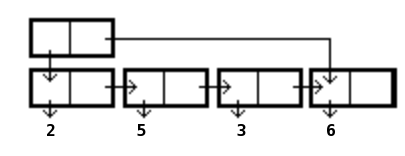
\includegraphics{DSAE1TwoCell.png}
\\ \newline
2
\\ \newline
[5, 3, 6]
\\ \newline
3

\section{Question 2}
\subsection{Brief}
In the lecture notes (Section 3.2) we looked at a procedure last(L) that returned the last item in the given list L. By performing the simplest possible modification of that procedure, create a recursive procedure secondlast(L) that returns the second to last item in a given list L.
\\ \newline
What is the time complexity of your algorithm?
\\ \newline
Now perform a more general modification of the last(L) procedure to give a recursive
procedure getItem(i,L) that returns the ith item in a list L, where i is an integer greater than zero.
\\ \newline

\subsection{Answer}
\begin{lstlisting}
let secondlast(L) =
    if isEmpty(L) then
        error "The list is Empty."
    else if isEmpty(rest(L)) then
        error "The list only has 1 element."
    else if isEmpty(rest(rest(L))) then
        return first(L)
    else
        return secondlast(rest(L))
\end{lstlisting}
Time Complexity : \textbf{O(n)}
\begin{lstlisting}
let getItem(i, L) =
    if i >= 0 then 
        error "i should be greater than 0."
    else if i = 1 then
        return first(L)
    else
        return getItem(i--, rest(L))
\end{lstlisting}

\section{Question 3}
\subsection{Brief}
It is often useful to know whether two given lists are the equal, i.e. contain the same items in the same order.  Write a recursive procedure equalList(L1,L2) that returns true if the two lists L1 and L2 are the same, and false if they are not. The only other procedures it may call are the standard primitive list operators \textit{first}, \textit{rest} and \textit{isEmpty}.
\\ \newline
What is the time complexity of your algorithm?
\subsection{Answer}
\begin{lstlisting}
let equallist(L1, L2) =
    if isEmpty(L1) xor isEmpty(L2) then
        false
    else
        return (first(L1) = first(L2)) and (equallist(rest(L1), rest(L2))
\end{lstlisting}
Time Complexity : \textbf{O(n)}

\section{Question 4}
\subsection{Brief}
A set can be represented as a list in which repeated items are not allowed and the order of the 2 items does not matter. Suppose you have sets S1 and S2 represented as linked-lists, and access to the standard list operators \textit{first}, \textit{rest}, and \textit{isEmpty}. 
\\ \newline
Write a recursive procedure member(x,S1) that returns true if item x is in set S1, and false if it is not.
\\ \newline
Now write a recursive procedure subset(S1,S2) that returns true if set S1 is a subset of set S2, and false if it is not.  It is only allowed to call the standard primitive list operators \textit{first}, \textit{rest} and \textit{isEmpty} and your \textit{member} procedure.
\\ \newline
Finally, write a procedure equalset(S1,S2) that returns true if set S1 is equal to set S2, and false if it is not.  It is only allowed to call the standard list operators \textit{first}, \textit{rest} and \textit{isEmpty} and your \textit{member} and \textit{subset} procedure.
\subsection{Answer}
\begin{lstlisting}
let member(x, S1) =
    if isEmpty(S1) then
        return false
    else if x = first(S1) then
        return true
    else
        return member(x, rest(S1))
        
let subset(S1, S2) = 
    if isEmpty(S1) then
        return true
    else if member(first(S1), S2) then
        return subset(rest(S1), S2)
    else
        return false
        
let equalset(S1, S2) = 
    return subset(S1, S2) and subset(S2, S1)
\end{lstlisting}
\end{document}